\documentclass[tikz,border=10pt]{standalone}
\usepackage{pgfplots}
\pgfplotsset{compat=1.18}
\begin{document}
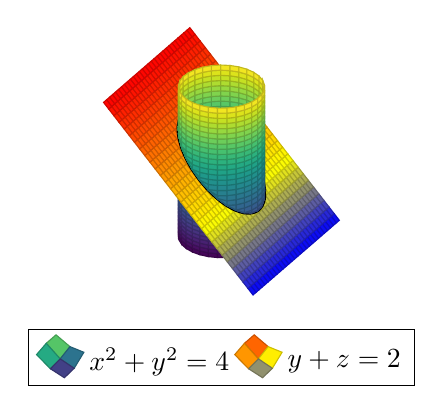
\begin{tikzpicture}
  \pgfplotsset{
    every axis legend/.append style={
      at={(0.5,0)},
      anchor=south,legend columns=2
    }}
  \begin{axis}[unit vector ratio=1 1 1, axis lines=none, view={120}{30}]
		
  % Parte inferior del cilindro
  % Min utiliza el menor valor entre el eje z sin parametrizar y la z parametrizada 
  \addplot3[surf,z buffer=sort,samples=30,colormap/viridis,
    variable=\u, variable y=\v,
    domain=0:360, y domain=0:3]
    ({cos(u)}, {sin(u)},{min(2-y,v)});		

  % Plano parametrizado y+z=2
  \addplot3[surf, z buffer=sort, samples=30,
    variable=\u, variable y=\v,domain=-2:2, y domain=-2:2]({u}, {v},{2-v});

  % Interseccion parametrizada
  \addplot3[color=black,smooth,samples=30,
     variable=\u,domain=0:360,line width=1.25pt]
    ({cos(u)}, {sin(u)},{2-sin(u)});

  % Parte superior del cilindro. Utiliza max tal en la parte inferior
  \addplot3[colormap/viridis,surf,z buffer=sort,samples=30,variable=\u, variable y=\v,
    domain=0:360, y domain=0:4]({cos(u)}, {sin(u)},{max(2-y,v)});
 
  % NOTA: el orden de dibujo de las superficies cambia si se aplica una vista diferente a la 120 30
  \legend{$x^2+y^2=4$,$y+z=2$}
  \end{axis}		
\end{tikzpicture}
\end{document}